\chapter{Clustering Algorithms for the Reconstruction of the CMS High Granularity Calorimeter (HGCAL)}
\label{sec:hgcal}


% phase II upgrade
The luminosity of the future High Luminosity Large Hadron Collider (HL-LHC) is going to achieve up to $7.5\times 10^{34}$ $\text{cm}^{-2}\text{s}^{-1}$ \cite{hllhcweb} in its ultimate scenario, which is 5 times that delivered at present. This leads to the production of high pile-up events containing up to 200 interactions in each bunch crossing (PU200). Current CMS endcap calorimeters \cite{Chatrchyan:2008aa} are designed with a lifetime radiation limit of 500 fb$^{-1}$ \cite{CMSCollaboration:2015zni}, which will be reached at the end of LHC Run-III in 2023. During the third long shutdown period of LHC from 2024 to 2026, the CMS Collaboration is going to conduct the Phase-II upgrade of the CMS detector \cite{CMSCollaboration:2015zni}. One of the major tasks in the CMS Phase-II upgrade is to replace the current endcap calorimeters, including both endcap electromagnetic and hadronic calorimeters, with a new high granularity calorimeter system (HGCAL) which is based on highly-segmented Silicon sensors and plastic scintillators.


The \BWl measurement presented in this thesis achieves 2\% relative uncertainty on the \BWt result. One of the most offending systematic uncertainties that limit the precision is the efficiency of hadronic identification, which has a 5\% relative uncertainty, about 1\% coming from the statistics of the measurement, 4\% coming from the systematics related to the track cuts of $\pt>0.5\GeV$. HGCAL is designed to make the most advantage of its fine channels to achieve the best possible spatial resolution, energy resolution and particle identification efficiency. It is able to detector photons and charged hadrons at much smaller separation, which is one of the key steps to reconstruct \PGth decay mode in the hadron-plus-strip algorithm. Furthermore, noval computer vision (CV) based deep learning particle identification is under developing, which aims at identifying particles directly from the images of candidate jets. Therefore, in the HL-LHC era, HGCAL is able to bring a noticeable improvement of \BWl precision.

In parallel with the \BWl analysis, I have been heavily involved in the clustering algorithm of the HGCAL reconstruction. This chapter summarizes my main R\&D work for the HGCAL clustering algorithm.




\section{Design and Reconstruction of the CMS HGCAL}
\label{sec:hgcal:design}


\begin{figure}[ht]
    \centering
    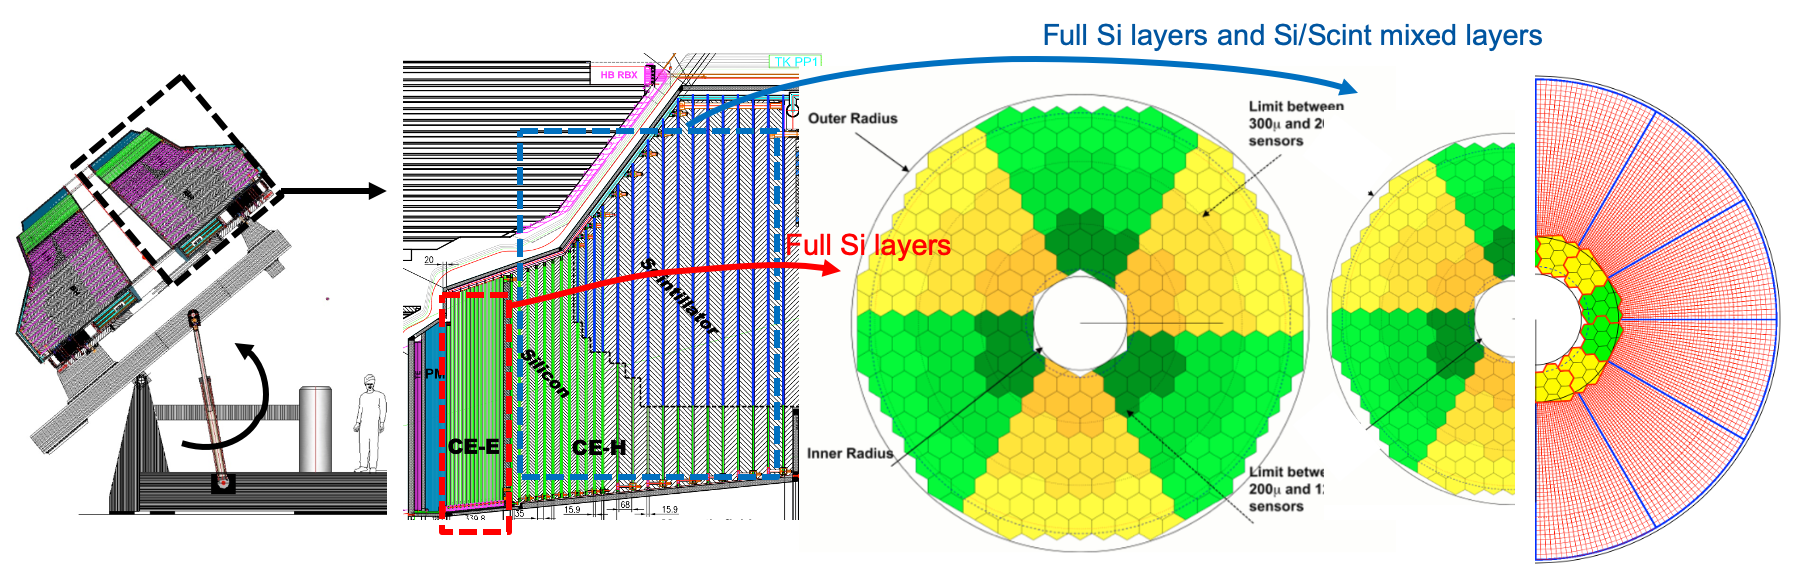
\includegraphics[trim=0cm 0cm 0cm 0cm, clip,width=0.99\textwidth]{chapters/HGCal/figures/chep/hgcal2.png} 
    \caption{ The design of HGCAL \cite{Collaboration:2293646}. (\emph{left}) Sketch of HGCAL endcap. (\emph{mid-left}) The internal structure on the longitudinal-radial (z-r) plane. Red and blue rectangles indicate regions of CE-E (for calorimeter endcap electromagnetic) and CE-H (for calorimeter endcap hadronic), respectively, where CE-E has 28 full Si layers and CE-H has 8 full Si layers plus 14 Si-scintillators hybrid layers. (\emph{mid-right, right}) Layouts of CE-E and CE-H layer. Silicon wafers are shown as yellow and green hexagons and scintillators are shown as red mesh. Darker, medium and lighter shades of hexagons represent silicon wafers with thickness of 120, 200 and 300 $\mu$m, respectively.
    }
    \label{fig:hgcal}
\end{figure}

% HGCAL design
The design of HGCAL \cite{Collaboration:2293646} is shown in Figure~\ref{fig:hgcal}. Two HGCAL endcaps will be mounted on both sides of the CMS detector. Each endcap weighs about 215 tons and measures about 2 m in longitudinal direction and 2.3 m in radial direction, covering $1.5<|\eta|<3.0$. The full system operates at a temperature of $-35^\circ$C maintained by a CO$_2$ cooling system. Each endcap consists of 50 layers, each of which combines passive absorber material and active sensor material. The front 28 layers are the electromagnetic part (CE-E), which uses Cu, CuW and Pb as absorber and Si wafers with 120, 200, 300 $\mu$m thickness as sensors. The back 22 layers are the hadronic part (CE-H), which uses stainless steel and Cu as absorber and includes 8 full Silicon layers plus 14 hybrid layers of Si sensors and plastic scintillators with SiPM readout. The electromagnetic radiation thickness and hadronic interaction thickness of CE-E are $25 X_0$ and $1.3 \lambda$ respectively, while the hadronic interaction thickness of CE-H is $8.2 \lambda$. In total, The full HGCAL system has 620 m$^2$ of Silicon and about 400 m$^2$ of plastic scintillators. The size of each Si sensor is 0.5-1.0 cm$^2$ and the number of Si channels is about 6 million. The size of the scintillators is 4-30 cm$^2$ and the number of scintillator channels is about 240 thousand.


% HGCAL reconstruction
As a consequence of both high pile-up in the HL-LHC and enormous number of channels in the HGCAL, the number of input hits to HGCAL clustering algorithm is huge, usually in the order of $n\sim O(10^5)$ in PU200 events, where $n$ denotes the number of hits. The clustering algorithm aggregates hits in 2D clusters layer by layer, producing about $k \sim O(10^4)$ clusters, where $k$ denotes number of clusters. The average number of hits in a cluster is about $m=n/k \sim 10$; therefore HGCAL clustering task is characterized by $n> k \gg m$. Since cells are small compared to shower lateral size, an "energy density" is defined to better hint regional energy blobs in the HGCAL clustering. After 2D clustering algorithm, 3D showers in HGCAL are reconstructed by collecting and associating 2D clusters on different layers using TICL algorithms \cite{ticlwebsite}. 

% time budget
The current trigger system in CMS consists of two levels: Level 1 Trigger (L1T) and High Level Trigger (HLT). L1T utilizes customized ASICs and FPGAs to reduce the event rate from 40 MHz LHC collision frequency to 100 kHz within a 4 $\mu$s time budget for decision; HLT is fully based on C++ software running on CPUs and further reduces event rate from 100 kHz to 1 kHz with a 300 ms time budget for decision. However, in the era of HL-LHC, CMS HLT expects 30 times more computing load: 1.3x from upgraded detectors with more channels; 3x from increased number of pile-up interactions; 7.5x from improved L1T output rate. Among this 30x surge of the computing demand, improvement in the CPU performance by 2026 is expected to account for only 4x. Therefore, there will be a considerable deficit of computing power if the HLT architecture remains unchanged in 2026. In the HL-LHC era, the HLT time budget for CMS HGCAL clustering is roughly estimated to be less than a few tens of milliseconds. It is particularly a huge challenge of computing for the HGCAL clustering algorithm to process $n\sim5\times10^5$ hits within such a limited time budget. To cope with this computing challenge, CMS is studying the feasibility of heterogeneous computing in HLT and offline reconstruction. With the support of CUDA \cite{nvidia2011nvidia} in the CMS software framework (CMSSW), it is possible to accelerate the HGCAL reconstruction with GPUs. 



\section{CLUE Clustering Algorithm}
\label{sec:algorithm}

Calorimeters with high lateral and longitudinal readout granularity, capable of providing a fine grained image of electromagnetic and hadronic showers, have been suggested for future high energy physics experiments \cite{calice2012calorimetry}. The  silicon sensor readout cells of the CMS endcap calorimeter (HGCAL) \cite{Collaboration:2293646} for HL-LHC \cite{Apollinari:2284929} have an area of about $1 \mathrm{cm}^2$.
When a particle showers, the deposited energy is collected by the sensors on the layers which the shower traverses. 
The purpose of the clustering algorithm when applied to shower reconstruction is to group together individual energy deposits (hits) originating from a particle shower. Due to the high lateral granularity, the number of hits per layer is large, and it is computationally advantageous to collect together hits in 2D clusters layer-by-layer \cite{Chen:2017btc} and then associate these 2D clusters, representing energy blobs, in different layers \cite{Collaboration:2293646}.



However, a computational challenge emerges as a consequence of the large data scale and limited time budget. %For example, clustering millions of hits in each event is tightly constrained by a millisecond-level execution time.
Coping with this challenge requires the clustering algorithm to be highly efficient while maintaining a low computational complexity. Furthermore, a linear scalability is strongly desired in order to avoid bottlenecking the performance of the entire event reconstruction.  Finally, it is highly preferable to have a fully-parallelizable clustering algorithm to take advantage of the trend of heterogeneous computing with hardware accelerators, such as graphics processing units (GPUs), achieving a higher event throughput and a better energy efficiency.



% input/output, characteristics
The input to the clustering algorithm is a set of $n$ hits, whose number varies from a few thousands to a few millions, depending on the longitudinal and transverse granularity of the calorimeter as well as on the number of particles entering the detector. The output is a set of $k$ clusters whose number is usually one or two order of magnitudes smaller than $n$ and in principle depends on both the number of incoming particles and the number of layers. Assuming that the lateral granularity of sensors is constant and finite, the average number of hits in clusters ($m=n/k$) is also constant and finite. For example, in the CMS HGCAL, $m$ is in the order of 10. This leads to the relation among the number of hits $n$, the number of clusters $k$, and the average number of hits in clusters $m$ as $n > k \gg m$.



Most well-known algorithms do not simultaneously satisfy the requirements on linear scalability and easy parallelization for applications like clustering hits in high granularity calorimeters, which is characterized by low dimension and $n > k \gg m$. It is therefore important to investigate new, fast and parallelizable clustering algorithms, as well as their optimized accompanying spatial index that can be conveniently constructed and queried in parallel.

In this paper, we describe a novel density-based clustering algorithm (CLUE: CLUsters of Energy) with linear scalability and easy parallelization. Its development was inspired by the work described in ref.~\cite{rodriguez2014clustering}. In Section~\ref{sec:algorithm}, we describe the CLUE algorithm and its accompanying spatial index. Then in Section~\ref{sec:implementation}, some details of GPU implementations are discussed. Finally, in Section~\ref{sec:performance} we present CLUE's ability on non-spherical cluster shapes and noise rejection, followed by its computational performance when executed on CPU and GPU with synthetic data, mimicking hits in high granularity calorimeters.



% ------------------------------------
% ------------------------------------

\subsection{algorithm}
% review of current popular method
Clustering data is one of the most challenging tasks in several scientific domains. The definition of cluster is itself not trivial, as it strongly depends on the context. Many clustering methods have been developed based on a variety of induction principles \cite{maimon2005data}. Currently popular clustering algorithms include (but are not limited to) partitioning, hierarchical and density-based approaches \cite{maimon2005data,han2011data}. Partitioning approaches, such as k-mean \cite{lloyd1982least}, compose clusters by optimizing a dissimilarity function based on distance. However, in the application to high granularity calorimeters, partitioning approaches are prohibitive because the number of clusters $k$ is not known a priori. Hierarchical methods make clusters by constructing a dendrogram with a recursion of splitting or merging. However, hierarchical methods do not scale well because each decision to merge or split needs to scan over many objects or clusters \cite{han2011data}. Therefore, they are not suitable for our application. Density-based methods, such as DBSCAN \cite{Ester:1996:DAD:3001460.3001507}, OPTICS \cite{Ankerst:1999:OOP:304182.304187} and Clustering by Fast Search and Find Density Peak (CFSFDP) \cite{rodriguez2014clustering}, group points by detecting continuous high-density regions. They are capable of discovering clusters of arbitrary shapes and are efficient for large spatial database. If a spatial index is used, their computational complexity is $O(n\log n)$ \cite{han2011data}. However, one of the potential weaknesses of the currently well-known density-based algorithms is that they intrinsically include serial processes which are hard to parallelize: DBSCAN has to iteratively visit all points within an enclosure of density-connectedness before working on the next cluster \cite{Ester:1996:DAD:3001460.3001507}; OPTICS needs to sequentially add points in an ordered list to obtain a dendrogram of reachability distance \cite{Ankerst:1999:OOP:304182.304187}; CFSFDP needs to sequentially assign points to clusters in order of decreasing density \cite{rodriguez2014clustering}. In the application to high granularity calorimeters, as discussed in Section~\ref{sec:introduction}, linear scalability and fully parallelization are essential to handle a huge dataset efficiently by means of heterogeneous computing.


% our method
In order to satisfy these requirements, we propose a fast and fully-parallelizable density-based algorithm (CLUE) inspired by CFSFDP. For the purpose of the algorithm, each sensor cell on a layer with its energy deposit is taken as a 2D point with an associated weight equaling to its energy value. As in CFSFDP, two key variables are calculated for each point: the local density $\rho$ and the separation $\delta$ defined in Equation~\ref{eqn:algorithm:defineRho} and \ref{eqn:algorithm:defineDelta}, where $\delta$ is the distance to the nearest point with higher density (``nearest-higher'') which is slightly adapted from that in CFSFDP in order to take advantage of the spatial index. Then cluster seeds and outliers are identified based on thresholds on $\rho$ and $\delta$. Differing from cluster assignment in CFSFDP, which sorts density and adds points to clusters in order of decreasing density, CLUE first builds a list of followers for each point by registering each point as a follower to its nearest-higher. Then it expands clusters by passing cluster indices from the seeds to their followers iteratively. Since such expansion of clusters is fully independent from each others, it not only avoids the costly density sorting in CFSFDP, but also enables a $k$-way parallelization. Unlike the noise identification in CFSFDP, CLUE rejects noise by identifying outliers and their iteratively descendant followers, as discussed in Section~\ref{sec:performance:clusteringResults}.

%%%%%%%%%%%%%%%%%%%%%
% Spatial Index with Grid
%%%%%%%%%%%%%%%%%%%%%

\subsubsection{Spatial index with fixed-grid}
Query of neighborhood, which retrieves nearby points within a distance, is one of the most frequent operations in density-based clustering algorithms. CLUE uses a spatial index to access and query spatial data points efficiently. Given that the physical layout of sensor cells is a multi-layer tessellation, it is intuitive to index its data with a fixed-grid, which divides the space into fixed rectangular bins \cite{bentley1979data,levinthal1966molecular}. Comparing with the data-driven structures such as KD-Tree \cite{Bentley:1975:MBS:361002.361007} and R-Tree \cite{Guttman:1984:RDI:971697.602266}, space partition in fixed-grid is independent of any particular distribution of data points \cite{rigaux2001spatial}, thus can be explicitly predefined before loading data points. In addition, both construction and query with a fixed-grid are computationally simple and can be easily parallelized. Therefore, CLUE uses a fixed-grid as spatial index for efficient neighborhood queries.


% search box
\begin{figure}[ht]
    \centering
    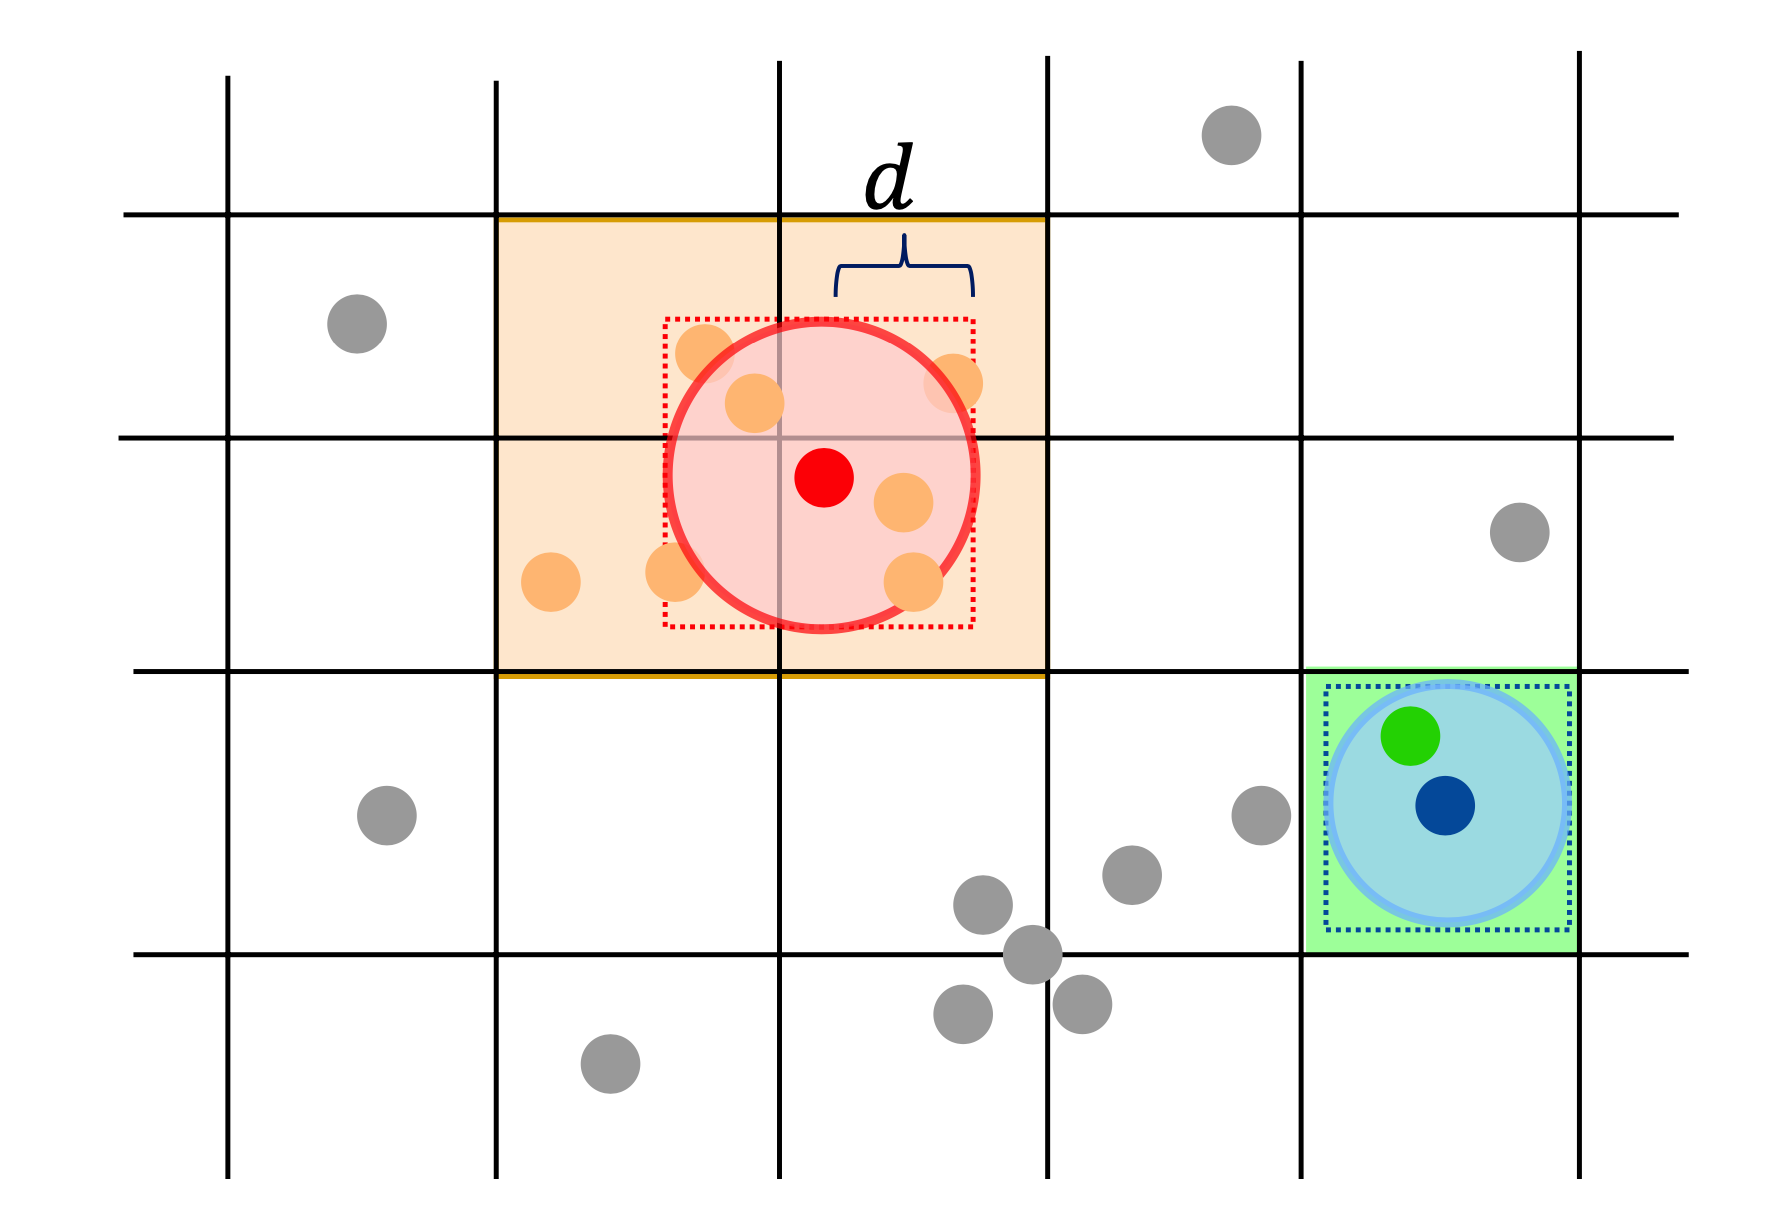
\includegraphics[width=0.4\textwidth]{chapters/HGCal/figures/clue/Figure1.png}
    \caption{2D points are indexed with a grid for fast neighborhood query in CLUE. Construction of this spatial index only involves registering the indices of points into the bins of the grid according to points' 2D spatial positions. To query d-neighborhood $N_d(i)$ defined in Equation~\ref{eqn:algorithm:defineNeighborhood}, taking the red (blue) point for example, we first locate its $\Omega_d(i)$ defined in Equation~\ref{eqn:algorithm:defineSearchBox}, a set of all points in the bins touched by a square window $[x_i\pm d,y_i\pm d]$. The $[x_i\pm d,y_i\pm d]$ window is shown as the orange (green) square while $\Omega_d(i)$ is shown as orange (green) points. Then we examine points in $\Omega_d(i)$ to identify those within a distance $d$ from point $i$, shown as the ones contained in the red (blue) circle.}
    \label{fig:algorithm:searchBox}
\end{figure}


For each layer of the calorimeter, a fixed-grid spatial index is constructed by registering the indices of 2D points into the square bins in the grid according to the 2D coordinates of the points. When querying $N_d(i)$, the d-neighborhood of point $i$, CLUE only needs to loop over points in the bins touched by the square window $(x_i\pm d,y_i\pm d)$ as shown in Fig.~\ref{fig:algorithm:searchBox}. We denote those points as $\Omega_d(i)$, defined as:
\begin{equation} \label{eqn:algorithm:defineSearchBox}
    \Omega_d(i) = \{j : j \in \textrm{tiles touched by the square window } [x_i\pm d,y_i\pm d] \}.
\end{equation}
\noindent where $\Omega_d(i)$ is guaranteed to include all neighbors within a distance $d$ from the point $i$. Namely, 
\begin{equation} \label{eqn:algorithm:defineNeighborhood}
    N_d(i)=\{j: d_{ij}<d, j \in \Omega_d(i) \} \subseteq \Omega_d(i).
\end{equation}
\noindent Without any spatial index, the query of $N_d(i)$ requires a sequential scan over all points. In contrast, with the grid spatial index, CLUE only needs to loop over the points in $\Omega_d(i)$ to acquire $N_d(i)$. Given that $d$ is small and the maximum granularity of points is constant, the complexity of querying $N_d(i)$ with a fixed-grid is $O(1)$.


%%%%%%%%%%%%%%%%%%%%%
% Parameters and Procedure
%%%%%%%%%%%%%%%%%%%%%

\subsubsection{Clustering procedure of CLUE}

CLUE requires the following four parameters: $d_c$ is the cutoff distance in the calculation of local density; $\rho_c$ is the minimum density to promote a point as a seed or the maximum density to demote a point as an outlier; $\delta_c$ and $\delta_o$ are the minimum separation requirements for seeds and outliers, respectively. The choice of these four parameters can be based on physics: for example, $d_c$ can be chosen based on the shower size and the lateral granularity of detectors; $\rho_c$ can be chosen to exclude noise; $\delta_c$ and $\delta_o$ can be chosen based on the shower sizes and separations. These four parameters allow more degrees of freedom to tune CLUE for the desired goals of physics. %, such as better energy resolution and better pile-up rejection.

\begin{figure}[ht]
    \centering
    \includegraphics[trim=5cm 0cm 4cm 0cm, clip,width=0.99\textwidth]{chapters/HGCal/figures/clue/Figure2.pdf}
    \caption{Demonstration of CLUE algorithm. Points are distributed inside a $6\times6$ 2D area and CLUE parameters are set to $d_c=0.5,\rho_c=3.9,\delta_c=\delta_o=1$. Before the clustering procedure starts, a fixed-grid spatial index is constructed. In the first step, shown as Fig.~\ref{fig:algorithm:procedure} (a), CLUE calculates the local density $\rho$ for each point, which is defined in Equation~\ref{eqn:algorithm:defineRho}. The color and size of points represent their local densities. In the second step, shown as Fig.~\ref{fig:algorithm:procedure} (b), CLUE calculates the nearest-higher $nh$ and the separation $\delta$ for each point, which are defined in Equation~\ref{eqn:algorithm:defineDelta}. The black arrows represent the relation from the nearest-higher of a point to the point itself. If the nearest-higher of a point is -1, there is no arrow pointing to it. In the third step, shown as Fig.~\ref{fig:algorithm:procedure} (c), CLUE promotes a point as a seed if $\rho,\delta$ are both large, or demote it to an outlier if $\rho$ is small and $\delta$ is large. Promoted seeds and demoted outliers are shown as stars and grey squares, respectively. In the fourth step, shown as Fig.~\ref{fig:algorithm:procedure} (d), CLUE propagates the cluster indices from seeds through their chains of followers defined in Equation~\ref{eqn:algorithm:defineFollowers}. Noise points, which are outliers and their descendant followers, are guaranteed not to receive any cluster ids from any seeds. The color of points represents the cluster ids. A grey square means its cluster id is undefined and the point should be considered as noise.
    }
    \label{fig:algorithm:procedure}
\end{figure}


% rho 
Figure~\ref{fig:algorithm:procedure} illustrates the main steps of CLUE algorithm. The local density $\rho$ in CLUE is defined as:
\begin{equation} \label{eqn:algorithm:defineRho}
    \rho_i = \sum_{j: j \in N_{d_c}(i)} \chi(d_{ij}) w_j,
\end{equation}
\noindent where $w_j$ is the weight of point $j$, $\chi(d_{ij})$ is a convolution kernel, which can be optimized according to specific applications. Obvious possible kernel options include flat, Gaussian and exponential functions. 

% delta
The nearest-higher and the distance to it $\delta$ (separation) in CLUE are defined as:
\begin{equation} \label{eqn:algorithm:defineDelta}
    nh_i = 
    \begin{cases}
        \arg\min_{j \in N'_{d_m}(i) } d_{ij},   & \text{if } |N'_{d_m}(i)| \neq 0  \\
        -1,                                     & \text{otherwise}
    \end{cases}, 
    \quad
    \delta_i = 
    \begin{cases}
        d_{i,nh_i}, & \text{if }  |N'_{d_m}(i)| \neq 0 \\
        +\infty,    & \text{otherwise}
    \end{cases},
\end{equation}
\noindent where $d_m= \max (\delta_o, \delta_c)$ and $N'_{d_m}(i) = \{ j : \rho_j > \rho_i, j \in N_{d_m}(i) \}$ is a subset of $N_{d_m}(i)$, where points have higher local densities than $\rho_i$. 

% expand clusters
After $\rho$ and $\delta$ are calculated, points with density $\rho>\rho_c$ and large separation $\delta>\delta_c$ are promoted as cluster seeds, while points with density $\rho<\rho_c$ and large separation $\delta>\delta_o$ are demoted to outliers. For each point, there is a list of followers defined as:
\begin{equation} \label{eqn:algorithm:defineFollowers}
    F_i = \{j : nh_j=i \}.
\end{equation}
\noindent The lists of followers are built by registering the points which are neither seeds nor outliers to the follower lists of their nearest-highers. The cluster indices, associating a follower with a particular seed, are passed down from seeds through their chains of followers iteratively. Outliers and their descendant followers are guaranteed not to receive any cluster indices from seeds, which grants a noise rejection as shown in Fig.~\ref{fig:performance:outlierCuts}. The calculation of $\rho, \delta$ and the decision of seeds and outliers both support $n$-way parallelization, while the expansion of clusters can be done with $k$-way parallelization.
% theoretical complexity
Pseudocode of CLUE is included in Appendix~\ref{app:pseudocode}.
% For each of the $n$ points, CLUE computes $\rho$, $\delta$, list of followers and cluster index with a constant complexity granted by grid spatial index, resulting in $O(n)$ computational complexity. Besides, the space complexity is also $O(n)$ because CLUE only keeps a few algorithmic variables for each of $n$ points and does not rely on any $n\times n$ matrix. 




% ------------------------------------
% ------------------------------------
\subsection{GPU Implementation}
\label{sec:implementation}

 To parallelize CLUE on GPU, one GPU thread is assigned to each point, for a total of $n$ threads, to construct spatial index, calculate $\rho$ and $\delta$, promote (demote) seeds (outliers) and register points to the corresponding lists of followers of their nearest-highers. Next, one thread is assigned to each seed, for a total of $k$ threads, to expand clusters iteratively along chains of followers. The block size of all kernels, which in practice does not have a remarkable impact on the speed performance, is set to 1024. In the test in Table~\ref{tbl:performance:breakdown}, changing the block size from 1024 to 256 on GPU leads to only about $0.14$~ms decrease in the sum of kernel execution times. The details of parallelism for each kernel are listed in Table~\ref{tbl:implementation:parallelism}. Since the results of a CLUE step are required in the following steps, it is necessary to guarantee that all the threads are synchronized before moving to the next stage. Therefore, each CLUE step can be implemented as a separate kernel. To optimize the performance of accessing the GPU global memory with coalescing, the points on all layers are stored as a single structure-of-array (SoA), including information of their layer numbers and 2D coordinates and weights. Thus points on all layers are input into kernels in one shot.


\begin{table}[t]
    \renewcommand{\arraystretch}{1.25}
    % \small
    \centering
    \begin{tabular}{l|l|c|c}
        \hline
        Kernels                                  & parallelism    & total threads & block size \\
        \hline
        build fixed-grid spatial index           & 1 point/thread & n             & 1024 \\
        calculate local density                  & 1 point/thread & n             & 1024 \\
        calculate nearest-higher and separation  & 1 point/thread & n             & 1024 \\
        decide seeds/outliers, register followers& 1 point/thread & n             & 1024 \\
        expand clusters                          & 1 seed/thread  & k             & 1024 \\
        \hline
    \end{tabular} 
    \caption{Kernels and Parallelism}
    \label{tbl:implementation:parallelism}
\end{table}


When parallelizing CLUE on GPU, thread conflicts to access and modify the same memory address in global memory could happen in the following three cases:

\begin{itemize}
    \item ~multiple points need to register to the same bin simultaneously;
    \item ~multiple points need to register to the list of seeds simultaneously;
    \item ~multiple points need to register as followers to the same point simultaneously.
\end{itemize}


\noindent Therefore, atomic operations are necessary to avoid the race conditions among threads in the global memory. During an atomic operation, a thread is granted with an exclusive access to read from and write to a memory location which is inaccessible to other concurrent threads until the atomic operation finishes. 
%Atomic operation allows each thread in the race of memory manipulation to exclusively conduct operations on a piece of memory until operation finishes.
This inevitably leads to some microscopic serialization among threads in race. The serialization in cases (i) and (iii) is negligible because bins are usually small as well as the number of followers of a given point. In contrast, serialization in case (ii) can be costly because the number of seeds $k$ is large. This can cause delays in the execution of kernel responsible for seed promotion. Since the atomic pushing back to the list of seeds is relatively fast in GPU memory comparing to the data transportation between host and device, the total execution time of CLUE still does not suffer significantly from the serialization in case (ii). The speed performance is further discussed in Section~\ref{sec:performance}.






% ------------------------------------
% ------------------------------------

\subsection{Performance Evaluation}
\label{sec:performance}

% Clustering Results
\subsubsection{Clustering results}
\label{sec:performance:clusteringResults}

% clustering on some non spherical topology
\begin{figure}[ht]
    \centering
    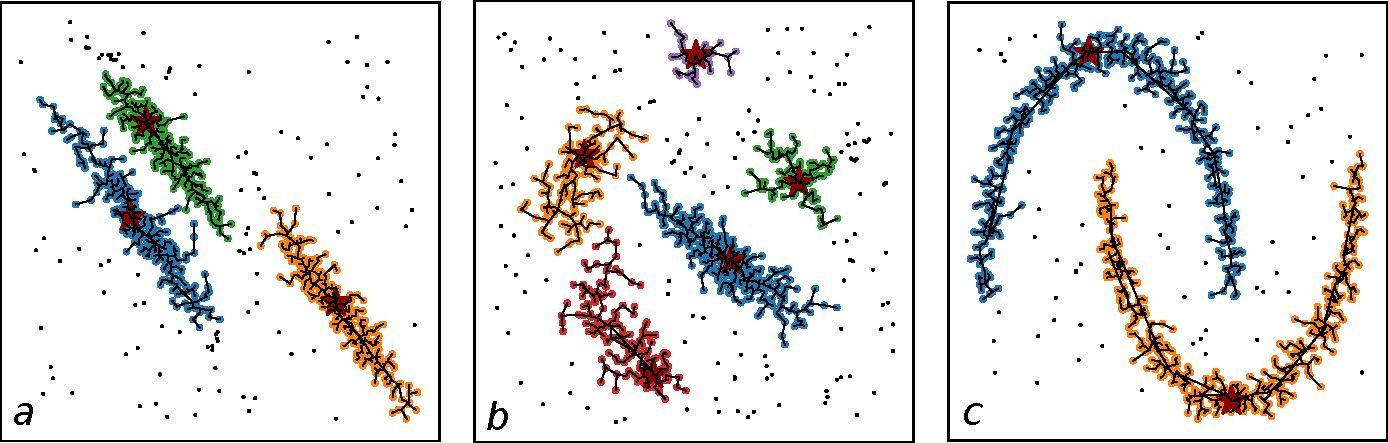
\includegraphics[clip, width=0.7\textwidth]{chapters/HGCal/figures/clue/Figure3_cut_boh.pdf}
    \caption{ 
    Examples of CLUE clustering on synthetic datasets. Each sample includes 1000 2D points with the same weight generated from certain distributions, including uniform noise points. The color of points represent their cluster ids. Black points represent outliers detached from any clusters. The links between pairs of points illustrate the relationship between nearest-higher and follower. The red stars highlight the cluster seeds.
    }
    \label{fig:performance:example}
\end{figure}

We demonstrate the clustering results of CLUE with a set of synthetic datasets, shown in Fig.~\ref{fig:performance:example}. Each example has 1000 2D points and includes spatially uniform noise points. The datasets in Fig.~\ref{fig:performance:example} (a) and (c)  are from the scikit-learn package~\cite{scikit-learn}. The dataset in Fig.~\ref{fig:performance:example} (b) is taken from~\cite{rodriguez2014clustering}. Fig~\ref{fig:performance:example} (a) and (b) include elliptical clusters and Fig~\ref{fig:performance:example} (c) contains two parabolic arcs. CLUE successfully detects
density peaks in Figs.~\ref{fig:performance:example} (a), (b), and (c).

\begin{figure}[ht]
    \centering
    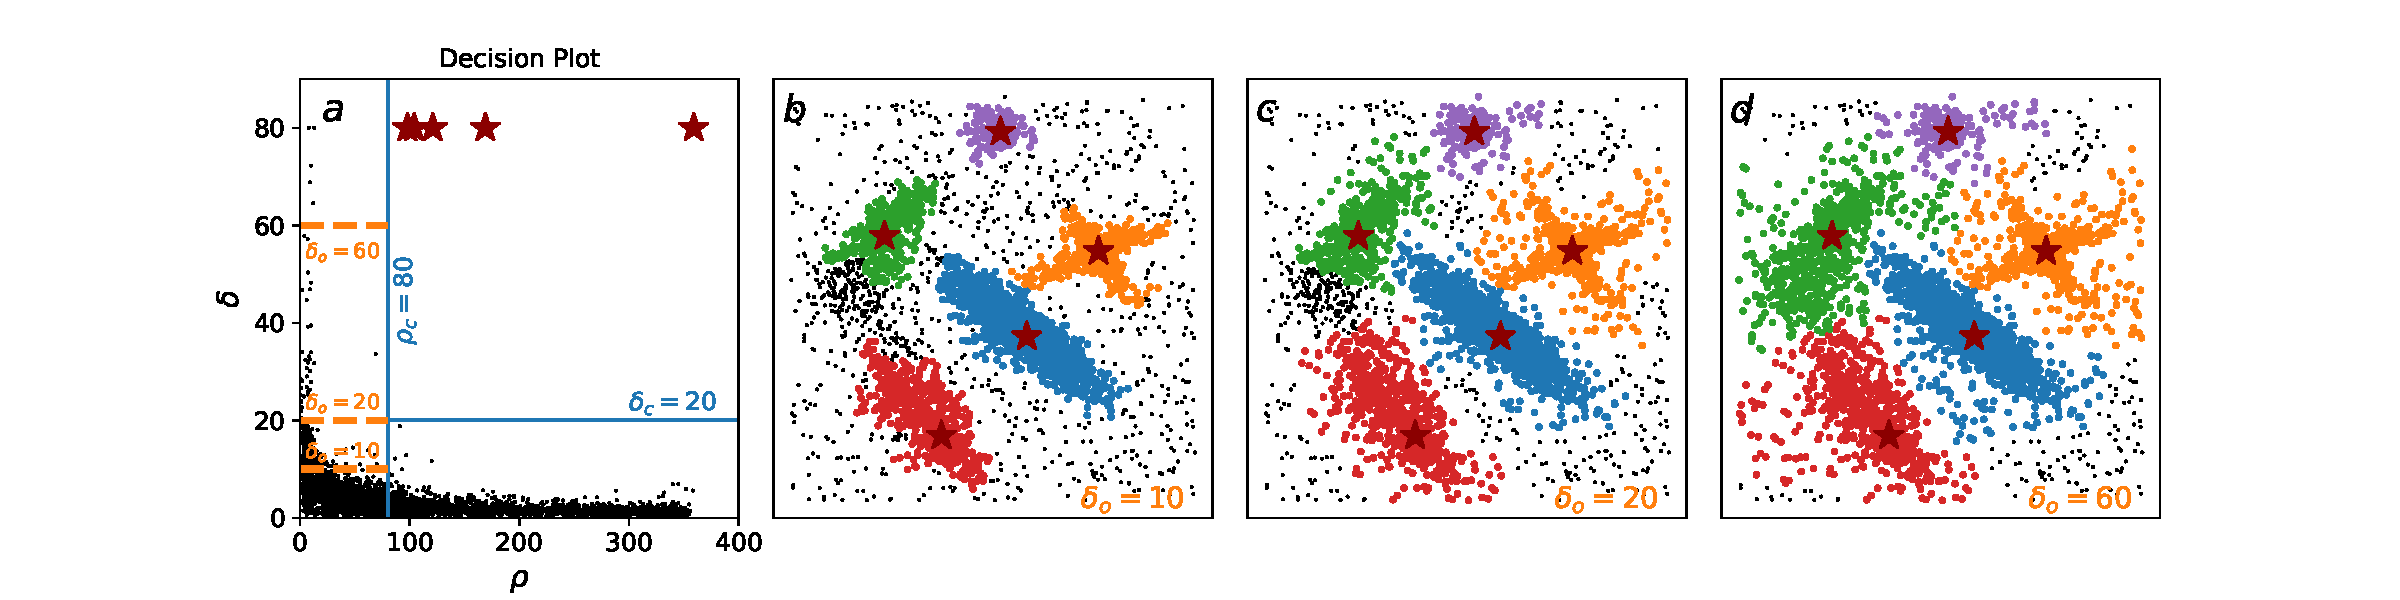
\includegraphics[trim=3.5cm 0cm 3.5cm 0cm, clip,width=0.99\textwidth]{chapters/HGCal/figures/clue/Figure4.pdf}
    \caption{ Noise rejection using different values of $\delta_o$. Noise is either an outlier or a descendant follower of an outlier. In this dataset~\cite{rodriguez2014clustering}, 4000 Points are distributed in $500\times500$ 2D square area. Figure~\ref{fig:performance:outlierCuts} (a) represents the decision plot on the $\rho-\delta$ plane, where fixed $\rho_c=80$ and $\delta_c=40$ values are shown as vertical and horizontal blue lines, respectively. Three different values of $\delta_o$ (10,20,60) are shown as orange dash lines. Figures~\ref{fig:performance:outlierCuts} (b), (c) and (d) show the results with $\delta_o=10,20,60$, respectively, illustrating how increasing $\delta_o$ loosens the continuity requirement and helps to demote outliers. The level of denoise should be chosen according to the user's needs.}
    \label{fig:performance:outlierCuts}
\end{figure}

In the induction principle of density-based clustering, the confidence of assigning a low density point to a cluster is established by maintaining the continuity of the cluster. Low density points with large separation should be deprived of association to any clusters. CFSFDP uses a rather costly technique, which calculates a boarder region of each cluster and defines core-halo points in each cluster, to detach unreliable assignments from clusters~\cite{rodriguez2014clustering}. In contrast, CLUE achieves this using cuts on $\delta_o$ and $\rho_c$ while expanding a cluster, as described in Section~\ref{sec:algorithm}. The example in Fig.~\ref{fig:performance:outlierCuts} shows how cutting at different separation values helps to demote outliers. Figure~\ref{fig:performance:outlierCuts} (a) represents the decision plot on the $\rho-\delta$ plane. Points with density below $\rho_c=80$, shown on the left side of the vertical blue line, could be demoted as outliers if their $\delta$ are larger than a threshold. Once an outlier is demoted, all its descendant followers are disallowed from attaching to any clusters. While keeping $\rho_c=80$ fixed, the effect of using three different values of $\delta_o$ (10, 20, 60), shown as orange dash lines in Fig.~\ref{fig:performance:outlierCuts} (a), has been investigated. The corresponding results are shown in Fig.~\ref{fig:performance:outlierCuts} (b),  (c) and (d), respectively.

% Scalability
\subsubsection{Execution time and scalability}
\label{sec:performance:executionTime}

\begin{figure}[ht!]
    \centering
    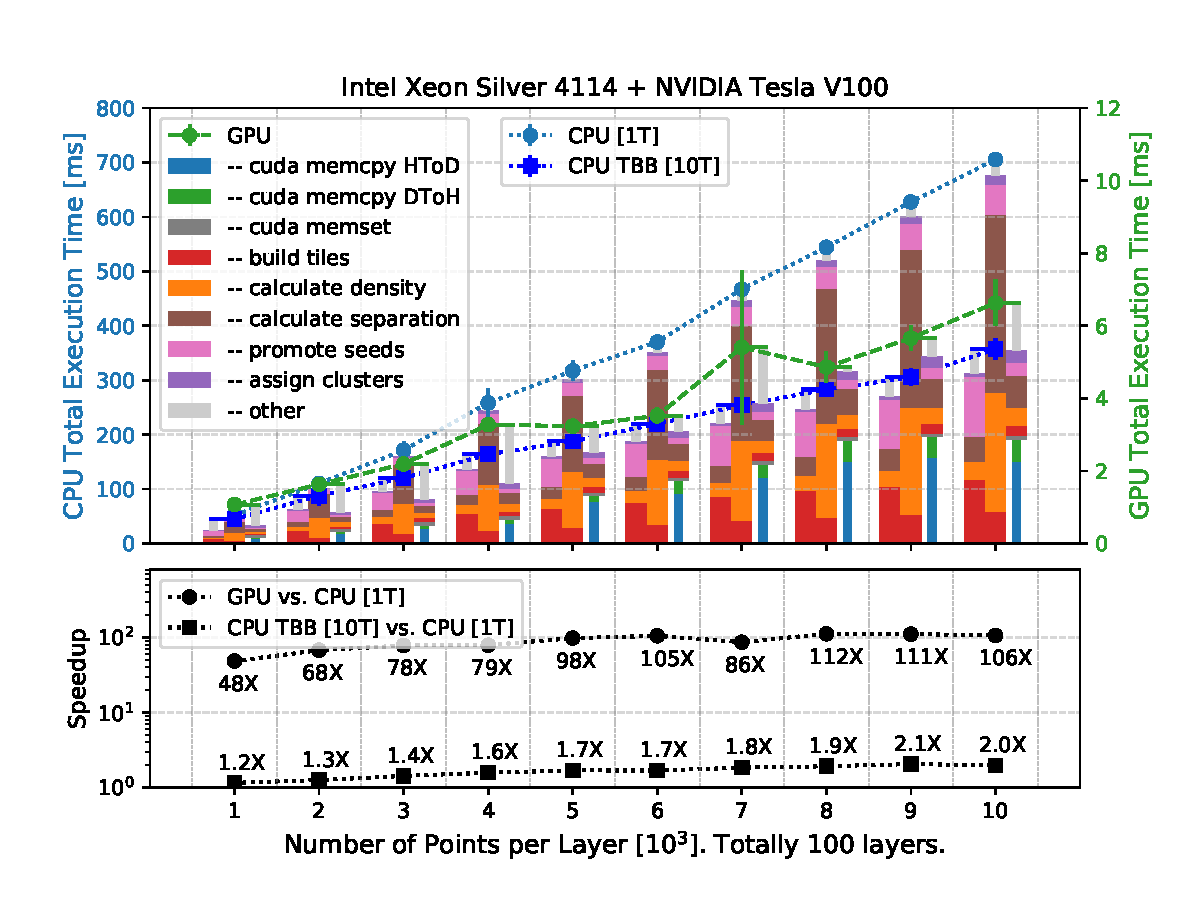
\includegraphics[width=0.9\textwidth]{chapters/HGCal/figures/clue/Figure5_patatrack02_1.pdf}
    \caption{ (\emph{Upper}) Execution time of CLUE on the single-threaded CPU, multi-threaded CPU with TBB and GPU scale linearly with number of input points, ranging from $10^5$ to $10^6$ in total. Execution time on single-threaded CPU is shown as blue circle dots and on 10 multi-threaded CPU with TBB is shown as blue square dots, while the time on GPU is shown as green circle dots. The stacked bars represent the decomposition of execution time. The green and blue narrower bars are latency for data traffic between host memory and device memory; wider bars represent time of essential CLUE steps; light grey narrower bars labelled as ``other'' are the difference between the total execution time and the sum of major CLUE steps (and major CUDA API calls if GPU). (\emph{Lower}) Comparing with the single-threaded CPU, the speedup factors of the GPU range from 48 to 112,  while the speedup factors of the multi-threaded CPU with TBB range from 1.2 to 2.0, which is less than the number of concurrent threads on CPU because of atomic pushing to the data containers discussed in Section~\ref{sec:implementation}. Table~\ref{tbl:performance:breakdown} shows the details of the decomposition of the execution time in the case of $10^4$ points per layer. }
    \label{fig:performance:executationTime}
\end{figure}

\begin{sidewaystable}[]
    \renewcommand{\arraystretch}{1.5}
    \caption{Decomposition of CLUE execution time in the case of $10^4$ points per layer with 100 layers. The time of sub-processes on GPU is measured with NVIDIA profiler, while on CPU is measured with \texttt{std::chrono} timers in the C++ code. The uncertainties are the standard deviations of 200 trial runs of the same event (10000 trial runs if GPU). The uncertainties of sub-processes on GPU are neglectable given that the maximum and minimum kernel execution time measured by NVIDIA Profiler are very close. With respect to the single-threaded CPU, the speedup factors of the multi-threaded CPU with TBB and the GPU are given in the bracket. ``other" represents the difference between total execution time and the sum of the execution time of CLUE steps (and major CUDA API calls if GPU).}
        
    % \tiny
    \centering
    % 10000
    \resizebox{0.9\textwidth}{!}{
    \begin{tabular}{l|r@{}l|r@{}l|r@{}l}
    \hline
    CLUE Step                                 & \multicolumn{2}{c}{CPU [1T] (baseline)}         & \multicolumn{2}{c}{CPU TBB [10T]}                    & \multicolumn{2}{c}{GPU}  \\ \hline
    build fixed-grid spatial index            &  59.3 $\pm$&  ~1.6 ms       & 117.7 $\pm$&  ~6.4 ms ( 0.50x)        &   0.28 ms& ~(208.63x)       \\
    calculate local density                   & 218.4 $\pm$&  ~2.5 ms       &  33.7 $\pm$&  ~2.6 ms ( 6.48x)        &   0.51 ms& ~(430.57x)       \\
    calculate nearest-higher and separation   & 326.9 $\pm$&  ~2.9 ms       &  45.5 $\pm$&  ~2.5 ms ( 7.19x)        &   0.89 ms& ~(368.54x)       \\
    decide seeds/outliers, register followers &  54.4 $\pm$&  ~2.5 ms       & 109.4 $\pm$&  ~7.7 ms ( 0.50x)        &   0.34 ms& ~(162.38x)       \\
    expand clusters                           &  17.4 $\pm$&  ~1.5 ms       &   6.1 $\pm$&  ~1.3 ms ( 2.86x)        &   0.35 ms& ~( 49.74x)       \\ \hline
    cuda memcpy                               & --&                         & --&                                  &   2.87 ms&                   \\ 
    cuda memset                               & --&                         & --&                                  &   0.10 ms&                   \\ 
    other                                     &  29.1 $\pm$&  ~1.7 ms       &  44.9 $\pm$& ~15.7 ms                 &   1.30 ms&                  \\ \hline
    \textbf{TOTAL} (10000 points per layer)   & \textbf{705.49 $\pm$}&  ~\textbf{7.93 ms} & \textbf{357.24 $\pm$}& ~\textbf{19.68 ms ( 1.97x)} & \textbf{  6.63 $\pm$ 0.63 ms}& ~\textbf{(106.42x)}  \\
    \hline
    \end{tabular}}

    \label{tbl:performance:breakdown}
\end{sidewaystable}


% testing dataset

We tested the computational performance of CLUE using a synthetic dataset that resembles high occupancy events in high granularity calorimeters operated at HL-LHC. The dataset represents a calorimeter with 100 sensor layers. A fixed number of points on each layer are assigned a unit weight in such a way that the density represents circular clusters of energy whose magnitude decreases radially from the centre of the cluster according to a Gaussian distribution with the standard deviation, $\sigma$, set to $3$~cm.
$5$\% of the points represent noise distributed
uniformly over the layers. When clustering with CLUE, the bin size is set to $5$~cm comparable with the width of the clusters and the
algorithm parameters are set to $d_c=3 \text{ cm},\delta_o=\delta_c=5 \text{ cm},\rho_c=8$. To test CLUE's linear scalability, the number of points on each layer is incremented from 1000 to 10000 in 10 equaling steps. A total of 100 layers are input to CLUE simultaneously which simulates the proposed CMS HGCAL design~\cite{Collaboration:2293646}. Therefore the total number of points in the test ranges from $10^5$ to $10^6$. 
%%The clustering result on toy dataset is included in the Appendix \ref{app:toyDetector}.
The linear scalability of execution time are validated in Fig.~\ref{fig:performance:executationTime}.



% testing software/hardware platform
The single-threaded version of the CLUE algorithm on CPU has been implemented in C++, while the one on GPU has been implemented in C with CUDA~\cite{nvidia2011nvidia}. The multi-threaded version of CLUE on CPU uses the Thread Building Block (TBB) library~\cite{reinders2007intel} and has been implemented using the Abstraction Library for Parallel Kernel Acceleration (Alpaka)~\cite{zenker2016alpaka}. The test of the execution time is performed on an Intel Xeon Silver 4114 CPU and NVIDIA Tesla V100 GPU connected by PCIe Gen-3 link. The time of each GPU kernel and CUDA API call is measured using the NVIDIA profiler. The total execution time is averaged over 200 identical events (10000 identical events if GPU). Since CLUE is performed event by event and it is not necessary to repeat memory allocation and release for each event when running on GPU, we perform a one-time allocation of enough GPU memory before processing events and a one-time GPU memory deallocation after finishing all events. Therefore, the one-time \emph{cudaMalloc} and \emph{cudaFree} are not included in the average execution time. Such exclusion is legit because the number of events is extremely massive in high energy physics experiments and the execution time of the one-time \emph{cudaMalloc} and \emph{cudaFree} reused by each individual event is negligible.




% performance result
In Fig.~\ref{fig:performance:executationTime} (\emph{upper}), the scalability of CLUE is linear, consistent with the expectation. The execution time on the single-threaded CPU, multi-threaded CPU with TBB and GPU increases linearly with the total number of points. The stacked bars represent the decomposition of execution time. In the decomposition, unique to the GPU implementation is the latency of data transfer between host and device, which is shown as blue and green narrower bars, while common to all the three implementations are the five CLUE steps. Comparing with the single-threaded CPU, when building spatial index and deciding seeds, shown as red and pink bars, the multi-threaded CPU using TBB does not give a notable speedup due to the implementation of atomic operations in Alpaka~\cite{zenker2016alpaka} as discussed in Section~\ref{sec:implementation}, while the GPU has a prominent outperformance thanks to its larger parallelization scale. For GPU, the kernel of seed promotion in which serialization exists due to atomic appending of points in the list of seeds, does not affect the total execution time significantly if compared with other sub-processes. In the two most computing-intense steps, calculating density and separation, there are no thread conflicts or inevitable atomic operations. Therefore, both the multi-threaded CPU using TBB and the GPU provide a significant speedup. The details of the decomposition of execution time in the case of $10^4$ points per layer are listed in Table~\ref{tbl:performance:breakdown}. 

Fig.~\ref{fig:performance:executationTime} (\emph{lower}) shows the speedup factors. Compared to the single-threaded CPU, the CUDA implementation on GPU is 48-112 times faster, while the multi-threaded version using TBB via Alpaka with 10 threads on CPU is about 1.2-2.0 times faster. The speedup factors are constrained to be smaller than the number of concurrent threads because of the atomic operations. In Table~\ref{tbl:performance:breakdown}, the speedup factors of multi-threaded CPU using TBB reduce to less than $1$ in the sub-process steps of building spatial index and promoting seeds and registering followers, where atomic operations happen and bottleneck the overall speedup factor.

\section{CLUE in the CMSSW}
\label{sec:cmsswClue}


The future High Luminosity LHC (HL-LHC) is expected to deliver about 5 times higher instantaneous luminosity than the present LHC, resulting in pile-up up to 200 interactions per bunch crossing (PU200). As part of the phase-II upgrade program, the CMS collaboration is developing a new end-cap calorimeter system, the High Granularity Calorimeter (HGCAL), featuring highly-segmented hexagonal silicon sensors and scintillators with more than 6 million channels. For each event, the HGCAL clustering algorithm needs to group more than $10^5$ hits into clusters. As consequence of both high pile-up and the high granularity, the HGCAL clustering algorithm is confronted with an unprecedented computing load. CLUE (CLUsters of Energy) is a fast fully-parallelizable density-based clustering algorithm, optimized for high pile-up scenarios in high granularity calorimeters. In this paper, we present both CPU and GPU implementations of CLUE in the application of HGCAL clustering in the CMS Software framework (CMSSW). Comparing with the previous HGCAL clustering algorithm, CLUE on CPU (GPU) in CMSSW is 30x (180x) faster in processing PU200 events while outputting almost the same clustering results.


\subsection{Implementation in the CMSSW}



% image algo
The previous clustering algorithm \cite{Chen:2017btc} used in the CMS HGCAL reconstruction was based on Clustering by Fast Search and Find Density Peak (CFSFDP) \cite{rodriguez2014clustering} and exploited a KD-Tree spatial index \cite{Bentley:1975:MBS:361002.361007}. In the step of calculating local density $\rho$, KD-Tree provides a significant speedup comparing with not using any spatial index \cite{Chen:2017btc}. However, it has three crucial computing weaknesses: first, KD-Tree does not provide the optimal spatial index for HGCAL, because its window-query is of $O(n\log n)$ complexity and it is hard to construct or query on the GPUs; second, the calculation of separation $\delta$ does not take advantage of spatial index but still relies on a costly $O(n^2)$ loop; third, the expansion of clusters happens in sequential order of decreasing density, which is not only costly because of sorting but also hard to parallelize.


% clue
CLUsters of Energy (CLUE) \cite{cluepaper} is a recently-proposed parallelizable high-speed clustering algorithm. It overcomes the above three computing weaknesses and achieves an average $O(n)$ computational complexity in the applications like HGCAL where $n> k \gg m$. CLUE uses a spatial index \cite{bentley1979data} for fast querying of neighbours. Figure \ref{fig:algorithm:procedure} is a demonstration of CLUE procedure provided in \cite{cluepaper}. Both the CPU and the GPU version of CLUE, referred as CLUE-CPU and CLUE-GPU in this paper, have been implemented in CMSSW for HGCAL reconstruction. CLUE-CPU is implemented in C++, while CLUE-GPU is implemented using CUDA. Figure~\ref{fig:cmssw} shows the workflow of CLUE-GPU within CMSSW: hits are offloaded from CPU to GPU after energy calibration; then CLUE steps are carried out on GPU; in the end, the clustering results are transported back to CPU for post processing and other downstream HGCAL reconstruction related to 3D linkage of CLUE clusters. 

% \begin{figure}[ht]
%     \centering
%     \includegraphics[trim=5cm 0cm 4cm 0cm, clip,width=0.99\textwidth]{chapters/HGCal/figures/chep/Figure2.pdf}
%     \caption{Demonstration of CLUE procedure \cite{cluepaper}. The definitions of four internal variables $\{ \rho, \delta, nh, followers\}$ are also given in \cite{cluepaper}. Before the clustering procedure starts, a fixed-grid spatial index is constructed. In the first step, shown as (a), CLUE calculates the local density $\rho$ for each point. The color and size of points represent their local densities. In the second step, shown as (b), for each point CLUE calculates its nearest-higher $nh$ (defined as the nearest hit with higher density) and its separation $\delta$ (defined as the distance to $nh$). The black arrows represent the relation from the nearest-higher of a point to the point itself. If the nearest-higher of a point is -1, there is no arrow pointing to it. In the third step, shown as (c), CLUE promotes a point as a seed if $\rho,\delta$ are both large, or demote it to an outlier if $\rho$ is small and $\delta$ is large. Promoted seeds and demoted outliers are shown as stars and grey squares, respectively. In the fourth step, shown as (d), CLUE propagates the cluster indices from seeds through their chains of followers. Noise points, which are outliers and their descendant followers, are guaranteed not to receive cluster ids from any seeds. The color of points represents the cluster ids. A grey square means its cluster id is undefined and the point should be considered as noise.
%     }
%     \label{fig:algorithm:procedure}
% \end{figure}


\begin{figure}[ht]
    \centering
    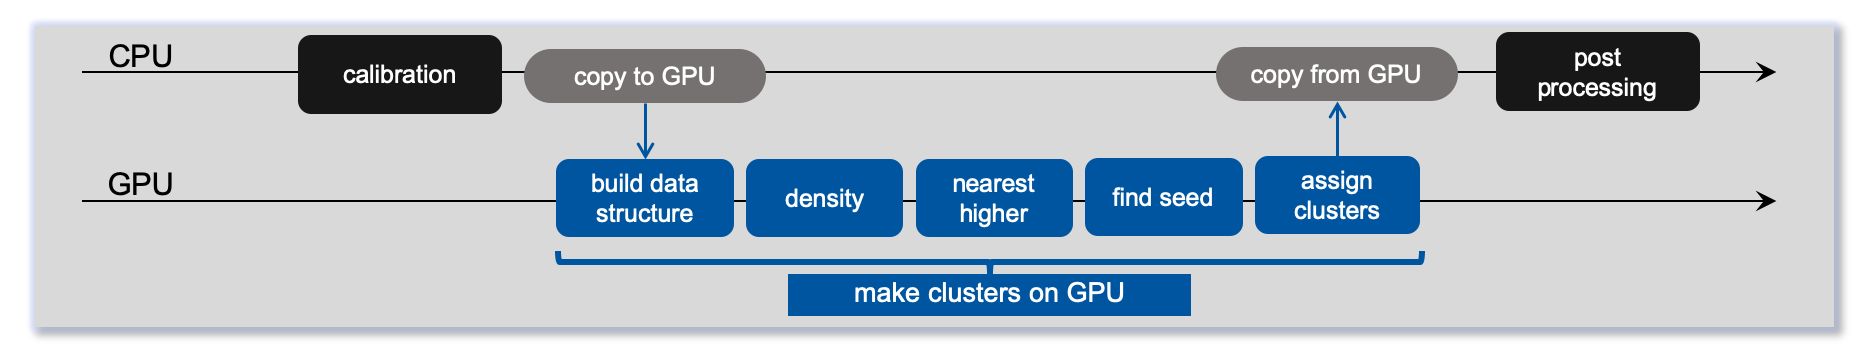
\includegraphics[trim=0.5cm 0cm 0.5cm 0cm, clip,width=0.99\textwidth]{chapters/HGCal/figures/chep/CMSSWFollow.png}
    \caption{ Workflow of CLUE-GPU in CMSSW. Hits are offloaded from CPU to GPU after energy calibration. Then CLUE process are carried out on GPU. In the end, the cluster indices of all hits are transported back to CPU for post processing.}
    \label{fig:cmssw}
\end{figure}


% validate CLUE result
\begin{figure}[ht]
    \centering
    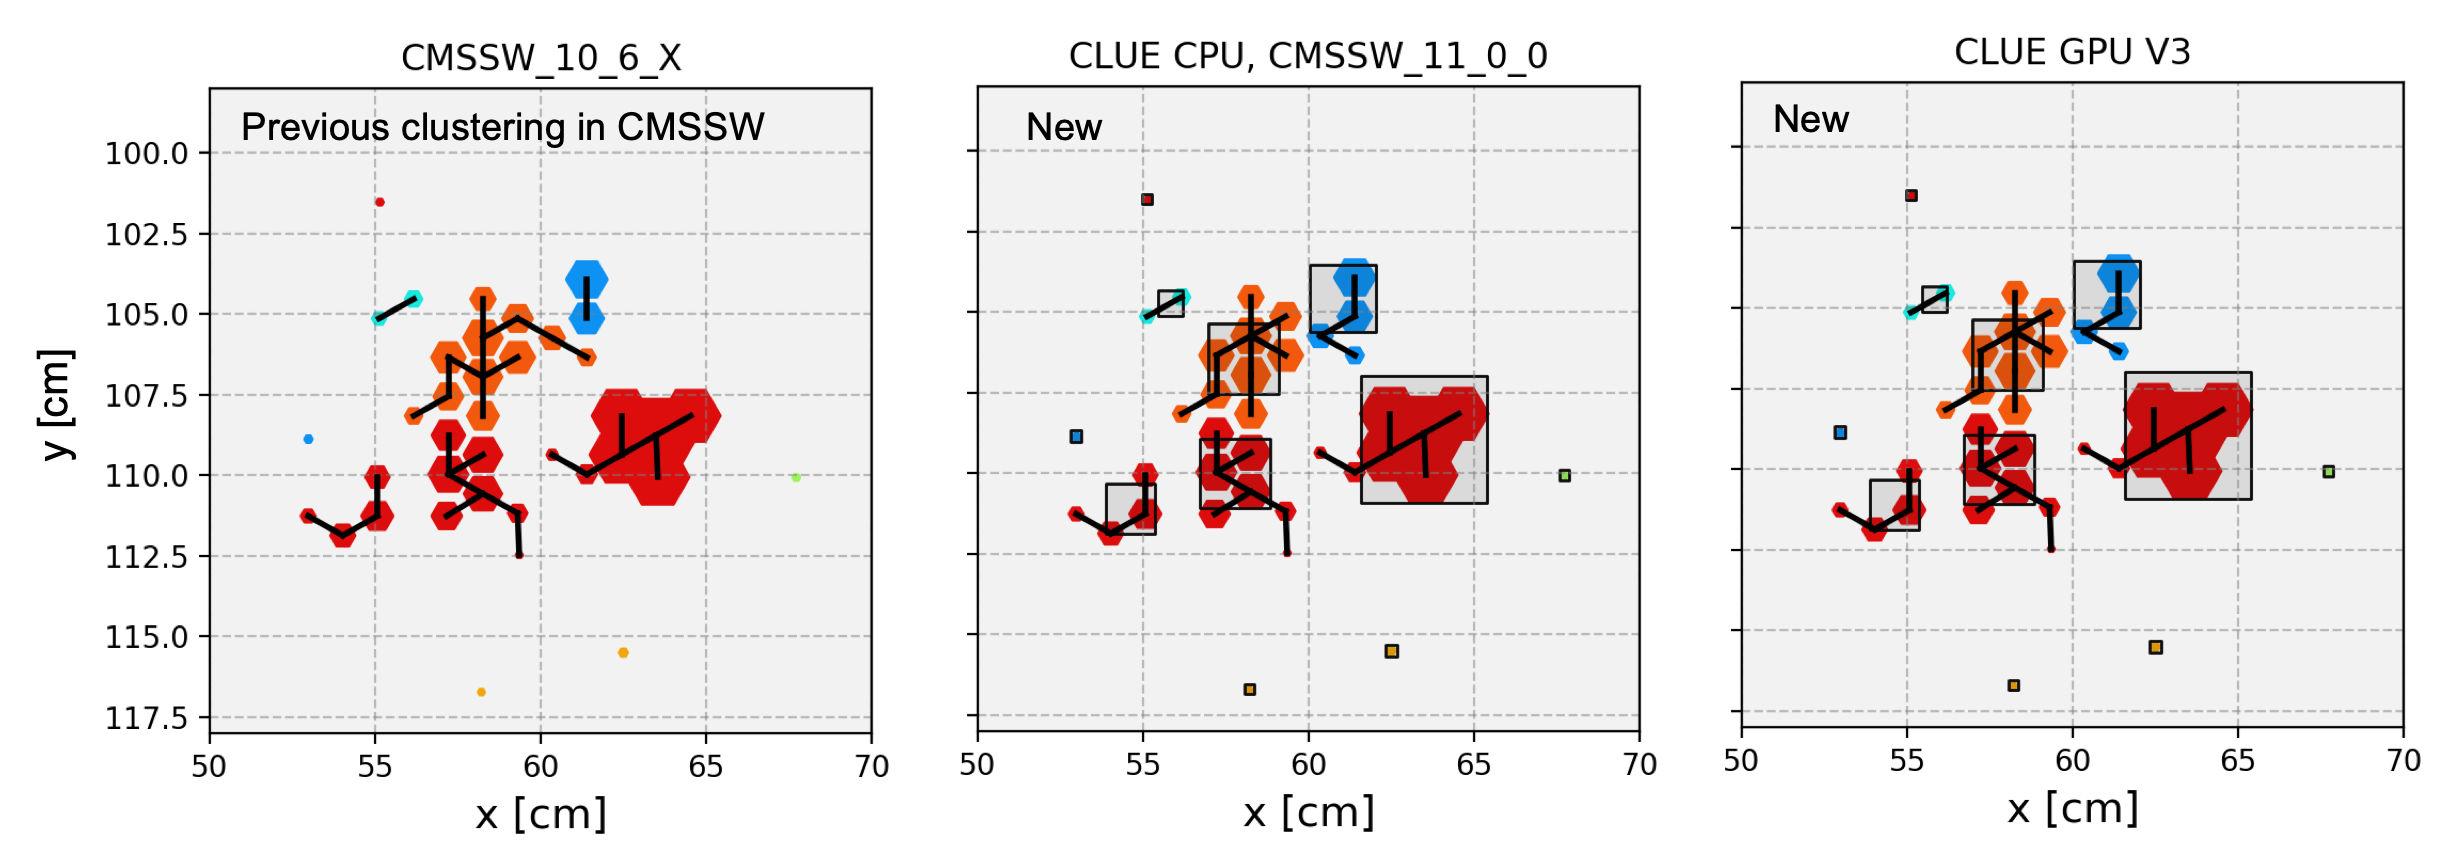
\includegraphics[trim=0cm 0cm 0cm 0cm, clip, width=0.90\textwidth]{chapters/HGCal/figures/chep/results.png}
    \caption{ Example of clustering result from previous algorithm in CMSSW\_10\_6\_X (\emph{left}) and CLUE-CPU (\emph{middle}) and CLUE-GPU (\emph{right}). The example shows a small region on the 12$^{th}$ layer of a simulated of $t\bar{t}$ event.
    }
    \label{fig:results}
\end{figure}

To validate the implementation of CLUE in CMSSW, results of CLUE-CPU and CLUE-GPU are compared with the previous clustering algorithm in CMSSW version 10.6, referred as CMSSW\_10\_6\_X. Based on the simulated $t\bar{t}$ events, CLUE-CPU and CLUE-GPU completely agree with each other, while both of them show some rare disagreements with the previous clustering algorithm implemented in CMSSW\_10\_6\_X. Such disagreements are caused by the different ordering of hits with exactly equal $\rho$ or equal $\delta$ when using different data structures, namely grid in CLUE and KD-Tree in CMSSW\_10\_6\_X. An example of clustering result is shown in Figure~\ref{fig:results}, where from left to right are results from CMSSW\_10\_6\_X, CLUE-CPU and CLUE-GPU. In this example, CLUE-CPU and CLUE-GPU provide almost the same result as the clusters in CMSSW\_10\_6\_X. However, a small notable difference is the blue cluster, which includes 4 hits in CMSSW\_10\_6\_X but 2 in CLUE. This is because the hit at about (x=60, y=106) cm is equally close to the two neighbouring hits in orange cluster and blue cluster, and its two different assignments, caused by different ordering of these two neighbors in spatial index, are equally correct. The topology of blue cluster in both cases are acceptable. Therefore, it is reasonable to conclude that CLUE in CMSSW gives almost the same clustering result as CMSSW\_10\_6\_X with neglectable differences.





\subsection{Performance in the CMSSW}


\begin{figure}[ht]
    \centering
    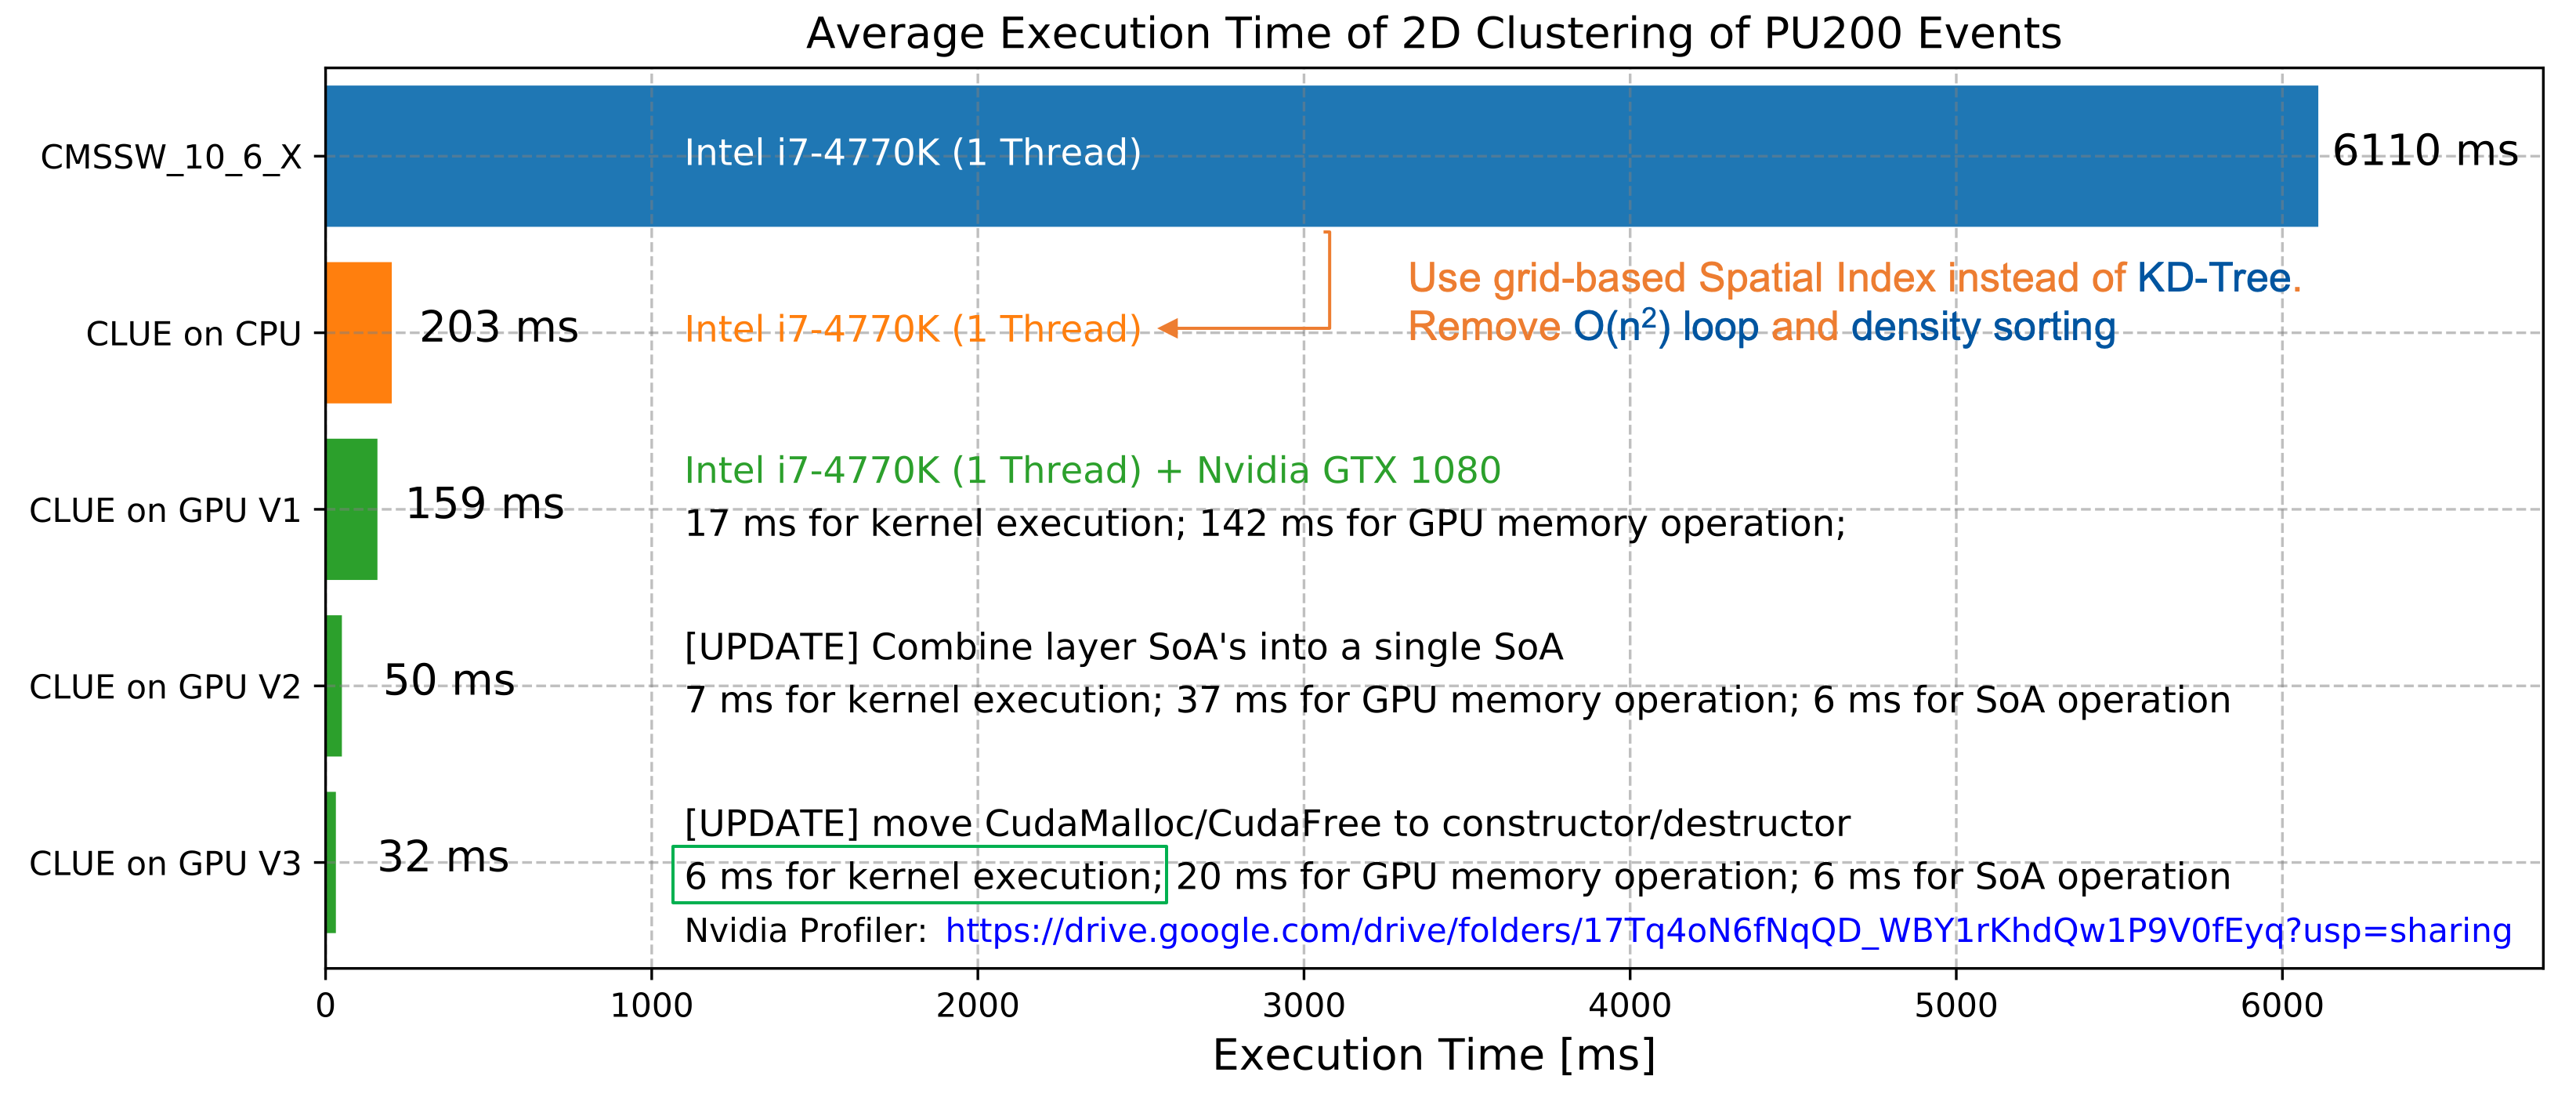
\includegraphics[trim=0cm 0cm 0cm 0cm, clip,width=0.99\textwidth]{chapters/HGCal/figures/chep/performance.png}
    \caption{ 
    Average execution time of HGCAL clustering for PU200 events. The testing platform is based on Intel i7-4770K CPU and NVIDIA GTX 1080 GPU. Blue, orange and green bars represent execution time of CMSSW\_10\_6\_X, CLUE-CPU and CLUE-GPU respectively. Both CMSSW\_10\_6\_X and CLUE-CPU use a single CPU thread. Three green bars are three evolving versions of CLUE-GPU and the most updated one is version 3 with 32 ms execution time, shown as the bottom-most green bar.
    }
    \label{fig:performance}
\end{figure}

The execution time of HGCAL clustering are tested using PU200 events. The testing platform is based on Intel i7-4770K CPU and NVIDIA GTX 1080 GPU. The average execution time is shown in Figure~\ref{fig:performance}, where measured time includes all clustering steps and all necessary data transfer between CPU and GPU. 

The previous clustering algorithm in CMSSW\_10\_6\_X using a single thread CPU takes 6110 ms on average. In comparison, CLUE-CPU takes only 203 ms using the same single thread CPU, producing almost the same result but 30x faster. The GPU implementation in CMSSW includes three versions. The first version is a plain CUDA implementation of CLUE-CPU and average execution time is 159 ms. The second version combines the data of all hits in the entire HGCAL as a single Structure of Array (SoA) to improve access to global memory and to allow parallelization of hits on different layers. The average execution time of the second version is reduced to 50 ms. The third version uses one-time GPU memory allocation and memory release before and after processing all events respectively. It further reduces execution time to 32 ms, which is decomposed into 6 ms for kernel execution, 20 ms for host-device data transportation and 6 ms for SoA conversion. The 6 ms total kernel execution time is comparable with that in \cite{cluepaper}. The speedup factor of CLUE-GPU over CLUE-CPU is about 6x. 

In the future, the latency due to data traffic and SoA conversion can be shared with other reconstruction processes if more processes are also offloaded to GPU. Such latency can also be partially hidden if multiple CUDA streams work on different events simultaneously to keep the GPU occupied.

% \section{TICL}
\label{sec:hgcal:reco}


The CMS endcap calorimeter upgrade for the High Luminosity LHC in 2027 uses silicon sensors to achieve radiation tolerance, with the further benefit of a very high readout granularity. Small scintillator tiles with individual SiPM readout are used in regions permitted by the radiation levels. A reconstruction framework is being developed to fully exploit the granularity and other significant features of the detector like precision timing, especially in the high pileup environment of HL-LHC. An iterative clustering framework (TICL) has been put in place, and is being actively developed. The framework takes as input the clusters of energy deposited in individual calorimeter layers delivered by the CLUE algorithm, which has recently been revised and tuned. Mindful of the projected extreme pressure on computing capacity in the HL-LHC era, the algorithms are being designed with modern parallel architectures in mind. Important speedup has recently been obtained for the clustering algorithm by running it on GPUs. Machine learning techniques are being developed and integrated into the reconstruction framework. This paper will describe the approaches being considered and show first results.



The reconstruction software in HGCAL is being developed with speed and portability in mind. The expected CPU trend in the next years will improve software performance by a factor~$ \sim3$~\cite{4}, while offline workflows and computing in CMS will require a factor~$ \sim30$, mainly driven by the reconstruction of simulated events~\cite{5}. In order to gain the missing factor~$ \sim10$ in performance, the HGCAL software reconstruction cannot rely on any other existing sub-detector software: this new detector represents a unique opportunity to exploit modern architectures and technologies. Therefore, two main solutions are being adopted to provide the needed improvements in CMS performance for Phase-2 runs: heterogeneous computing and machine learning. On the hardware side, GPUs have shown great results in terms of speedup in recent years and the use of hybrid architectures is spreading in many fields of science. In addition, NVIDIA GPUs can be programmed with CUDA (Compute Unified Device Architecture), a parallel computing platform and programming model designed to work with programming languages such as C, C++, Fortran and Python, allowing to easily accelerate compute intensive portions of the applications~\cite{6}. On the software side, machine learning models are largely exploited to accomplish an enormous variety of tasks and can provide better results than traditional methods in many cases. Furthermore, some machine learning algorithms (e.g. Convolutional Neural Networks) can be executed on GPU, thus reducing both training and inference times, thanks to frameworks like Tensorflow~\cite{7} and Keras~\cite{8}.

\subsection{TICL: The Iterative CLustering}
The development of the HGCAL reconstruction software is driven by three main concepts:
\begin{enumerate}
\itemsep0em
    \item Particles deposit energy and create \emph{RecHits};
    \item \emph{RecHits} on each layer are clustered together to form \emph{LayerClusters} (2D objects);
    \item \emph{LayerClusters} are linked together to form \emph{Tracksters}, collections of \emph{LayerClusters}.
\end{enumerate}

In order to build the reconstruction chain exploiting the full potential of HGCAL, a modular framework has been developed and is constantly evolving. TICL (The Iterative CLustering)~\cite{9} modules and interfaces are defined such that new developers don't need a deep knowledge of the official CMS software core framework (CMSSW) and can easily contribute. In addition, its flexibility and modularity allow users to test their own algorithms and compare performances, as they can be plugged on top of the framework without applying any strong modification to the existing workflow. The design of TICL framework is shown in Figure~\ref{fig:ticl}. The next sections will focus on the aforementioned three main aspects of TICL reconstruction. First, a typical TICL iteration that links \emph{LayerClusters} together to produce \emph{Tracksters} will be described in Section~\ref{sec:iter}. The 2D clustering procedure with CLUE algorithm is then presented in Section~\ref{sec:clue}; finally, preliminary results of particle identification and energy regression performed on a \emph{Trackster} with a Convolutional Neural Network are shown in Section~\ref{sec:pid}.

\begin{figure}[tbp]
    \centering % \begin{center}/\end{center} takes some additional vertical space
    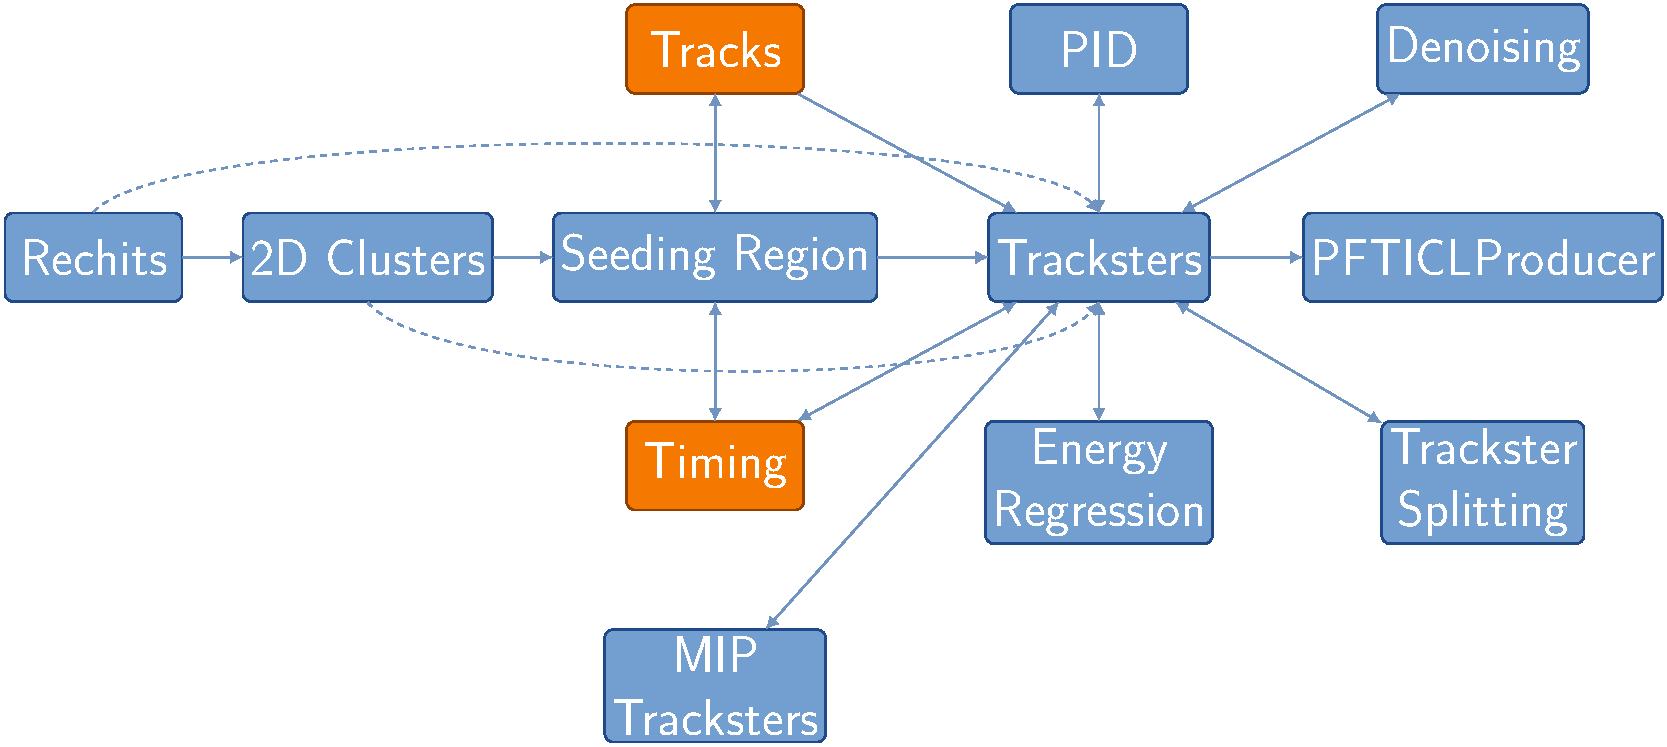
\includegraphics[width=.9\textwidth]{chapters/HGCal/figures/chef/ticl.pdf} 
    \caption{\label{fig:ticl} Design of TICL framework. Arrows show connections between different parts of the reconstruction, pointing from the output of a step to the input of a next step. Double pointing arrows indicate a strong connection between two parts of the reconstruction. \emph{Tracks} and \emph{Timing} (orange cells) are information coming from other subdetectors (respectively Tracker and MTD)~\cite{9}.}
\end{figure}

\subsection{TICL iterations}
\label{sec:iter}
\emph{Tracksters} produced by TICL iterations are suitable for representing real physics objects (i.e. particle showers). In order to guarantee such a correspondence, it's necessary to build a reconstruction workflow that takes into account the specific physics process that different particles undergo into the detector (hadronic and electromagnetic shower development, minimum ionizing particles, e.g. muons, etc.). Four different types of iteration exist now in TICL: \emph{track-seeded} (collects information from the Tracker to get the entry point and momentum direction of charged particles at the front face of the HGCAL detector), \emph{MIP} (\emph{Minimum Ionizing Particle}), \emph{electromagnetic} and \emph{hadronic}. The structure of a TICL iteration is shown in Figure~\ref{fig:iter}. A seeding region is first defined as a window in the [$\eta$, $\phi$] space on a certain layer and a pattern recognition algorithm is applied to all the available \emph{LayerClusters} within the seeding region. Then, linking, cleaning and classification tasks follow, exploiting timing information when possible. At the end of each iteration, the \emph{Tracksters} are required to pass quality criteria and particle identification: all the \emph{LayerClusters} belonging to the selected \emph{Tracksters} are masked out and are not available for the next iteration.

\begin{figure}[tbp]
    \centering % \begin{center}/\end{center} takes some additional vertical space
    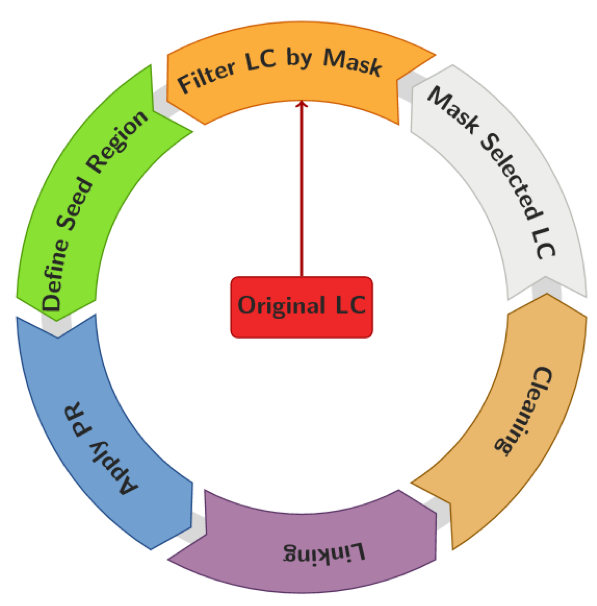
\includegraphics[width=.4\textwidth]{chapters/HGCal/figures/chef/iter}
    \qquad
    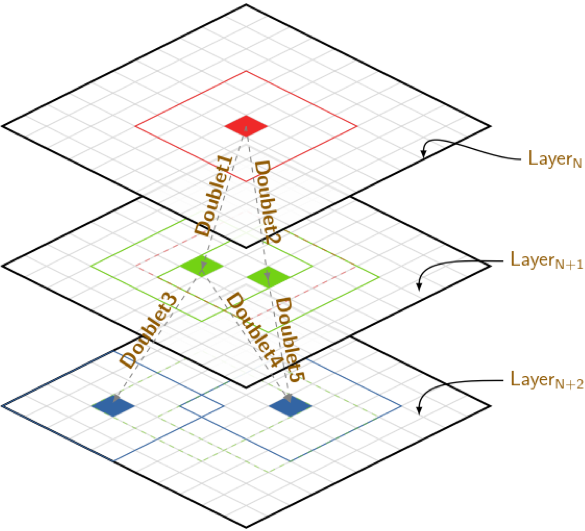
\includegraphics[width=.4\textwidth]{chapters/HGCal/figures/chef/pralgo}
    % "\includegraphics" from the "graphicx" permits to crop (trim+clip)
    % and rotate (angle) and image (and much more)
    \caption{\label{fig:iter} (\emph{Left}) Structure of a typical iteration in TICL. (\emph{Right}) Scheme of \emph{Cellular Automaton} pattern recognition implemented in TICL~\cite{9}.}
\end{figure}

Thanks to the modular design of the framework, several pattern recognition algorithms can be tested to produce the best results. Currently, a \emph{Cellular Automaton} algorithm is being used based on the experience with CMS Track reconstruction~\cite{10}. It consists of six main steps:

\begin{enumerate}
\itemsep0em
    \item Start from a Layer\textsubscript{N} and consider a specific \emph{LayerCluster}
    \item Open a window in the [$\eta$, $\phi$] space around it and project it onto the next Layer\textsubscript{N+1}
    \item Consider all the \emph{LayerClusters} inside this region and try to establish a \emph{Doublet} connection between the \emph{LayerClusters} on the two adjacent layers
    \item Apply some compatibility criteria to decide if the \emph{LayerClusters} should be linked or not (i.e. geometry constraints, energy, timing compatibility, etc.)
    \item Repeat this same procedure for all the \emph{LayerClusters} on Layer\textsubscript{N}
    \item Repeat this same procedure for all pairs of contiguous layers [Layer\textsubscript{K}, Layer\textsubscript{K+1}]
\end{enumerate}

At the end of the process, pairs of \emph{LayerClusters} will be connected into \emph{Doublets}. Consecutive \emph{Doublets} (i.e. doublets that share the ``middle'' \emph{LayerCluster}) will be linked together if configurable alignment requirements are satisfied. The set of all connected \emph{Doublets} will form a direct acyclic graph that serves as building block for a \emph{Trackster}. Note that this procedure can be properly configured to allow missing consecutive \emph{LayerClusters} and establish links between non-adjacent layers (e.g. in \emph{MIP} iteration). 


\subsection{Particle identification and energy regression}
\label{sec:pid}
The final purpose of the TICL framework is to reconstruct physics objects and energies and, at the same time, give probabilities on particle identification. To accomplish this task, some preliminary studies were conducted with a single particle produced in front of HGCAL in events where no pile-up is simulated. The momentum of the particle pointed from the vertex (0,0,0), center of the CMS detector. Events were simulated in such a way that particle showers (in case of electrons, photons and charged hadrons) could be fully contained inside the detector.

Since \emph{Tracksters} are suitable for representing real physics objects, a Convolutional Neural Network was designed to perform particle identification and energy regression on \emph{Tracksters} built by TICL electromagnetic iterations. In order to have fixed-sized inputs to the network, each \emph{Trackster} is represented as an image $50 \times 10 \times 3$, where the dimensions represent respectively the number of HGCAL layers per endcap, the maximum number of \emph{LayerClusters} on each layer and the number of features (energy, $\eta$, $\phi$). In this representation, each pixel of the image corresponds to a \emph{LayerCluster} that belongs to the \emph{Trackster}. Furthermore, \emph{LayerClusters} on each layer have been sorted by decreasing energy, applying a zero-padding whenever a layer featured less than 10 clusters, while removing some low energy \emph{LayerClusters} in layers with more than 10.

\begin{figure}[t]
    \centering
    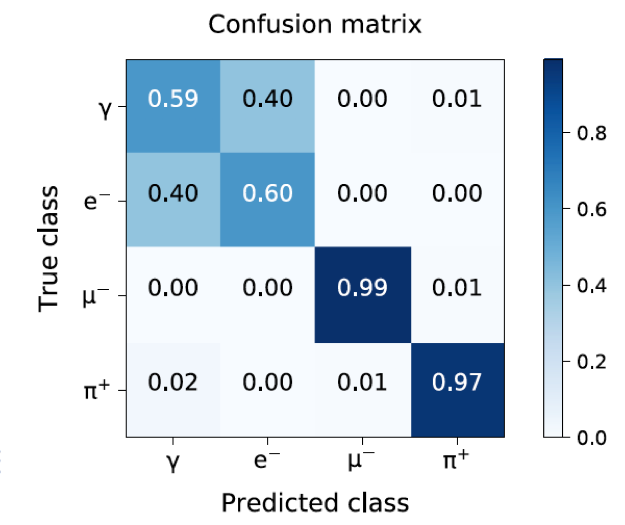
\includegraphics[width=.4\textwidth]{chapters/HGCal/figures/chef/pid}
    \caption{\label{fig:pid} Confusion matrix showing the performance of particle identification.}
\end{figure}

\begin{figure}[h]
    \centering
    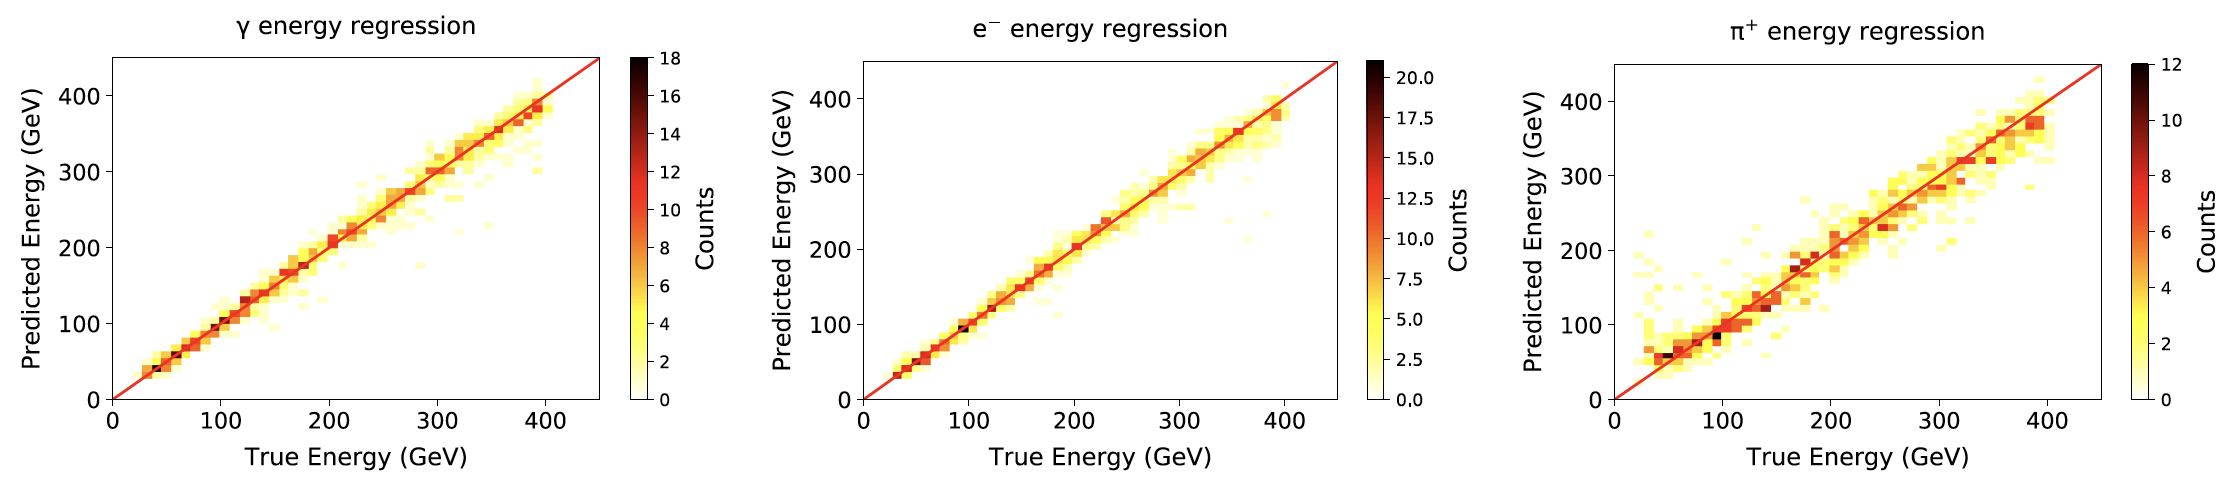
\includegraphics[width=.99\textwidth]{chapters/HGCal/figures/chef/er}
    \caption{\label{fig:er} Energy regression preliminary results for photons, electrons and charged hadrons.}
\end{figure}

A preliminary performance study was conducted on a 4-classes model (electron, photon, muon, charged hadron). The dataset consisted of 40 thousand events (10 thousand per particle type): $80\%$ has been used for training, $10\%$ for validation and the remaining $10\%$ for testing. The CNN was trained for 15 epochs (passes of the algorithm through the entire dataset), using the sum of cross-entropy and mean squared error as loss function to account for particle ID and energy regression, respectively. In order to have the value of the two functions of the same order of magnitude during training, the energies of the \emph{Tracksters} were normalized with respect to the data sample. The CNN was trained with Tensorflow~\cite{7}. Results are shown in Figure~\ref{fig:pid} and Figure~\ref{fig:er}. The confusion between electrons and photons is expected to be solved in future by exploiting information coming from the Tracker. The energy regression must be fine tuned and improvements are needed especially in the case of charged hadrons, since part of the shower is reconstructed by hadronic iteration. More classes will be added and the evolution of TICL is expected to improve the performance of this task.





